\section{Actividad 6}
\bigskip

	Considerar el diagrama ilustrado en la Fig. \ref{sistema}. Se tiene la primera etapa con un filtro
	pasa banda, al cual ingresa ruido blanco Gaussiano, de media cero y densidad espectral
	de potencia N0/2. Seguido a ello se tiene un modulador producto y finalmente un filtro
	pasa bajo. Las respuestas en frecuencia de ambos filtros pueden observarse en las Fig. \ref{pasabanda} y Fig. \ref{pasabajo}.


	\begin{figure}[H]
		\centering
		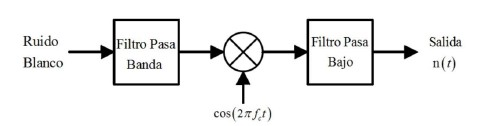
\includegraphics[width=12cm]{act_4_sistema.jpg}
		\caption{Esquema de la actividad 6.}
		\label{sistema}
	\end{figure}

	\begin{figure}[H]
		\centering
		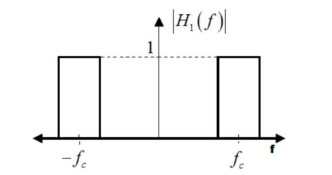
\includegraphics[width=6cm]{act4_pasabanda.jpg}
		\caption{Respuestas en frecuencia del filtro pasa banda.}
		\label{pasabanda}
	\end{figure}

	\begin{figure}[H]
		\centering
		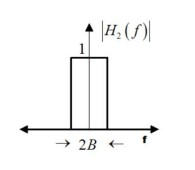
\includegraphics[width=4cm]{act_4_pbajos.jpg}
		\caption{Respuestas en frecuencia del filtro pasa bajo.}
		\label{pasabajo}
	\end{figure}



\noindent a) Calcular la densidad espectral de potencia y la función autocorrelación de $n(t)$. Graficar que se obtiene a la salida de cada filtro y del modulador producto (no debe usar el programa). \par
\bigskip

	\noindent La densidad espectral de potencia del ruido $n(t)$ en la salida del filtro pasabanda es:
		\[
				S_{NP_{Banda}}(f) =
				\begin{cases}
				\dfrac{N_0}{2} & -f_c - B < f < -f_c + B \\[6pt]
				\dfrac{N_0}{2} & f_c - B < f < f_c + B \\[6pt]
				0 & \text{o.c.}
				\end{cases}
		\]

	\noindent El gráfico de la densidad espectral de potencia a la salida del filtro pasabanda se observa en la Fig. \ref{fig:6pasabanda}.

		\begin{figure}[H]
			\centering
			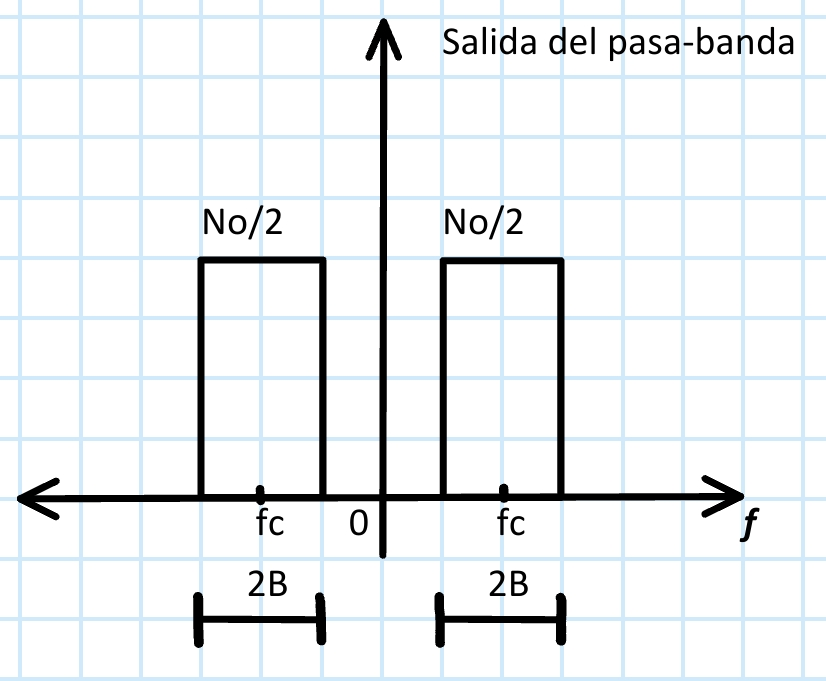
\includegraphics[width=7cm]{parte_teorica/actividad6_pasabanda.jpg}
			\caption{Densidad espectral de potencia del filtro pasabanda.}
			\label{fig:6pasabanda}
		\end{figure}


	\noindent Luego, la salida del filtro pasabanda se multiplica por la señal portadora $\cos(2 \pi f_c t)$, donde la transformada de Fourier de dicha portadora es:
		\[
			\cos(2 \pi f_c t) = \tfrac{1}{2} \left[ \delta(f - f_c) + \delta(f + f_c) \right]
		\]
	
	\noindent Al multiplicar en el dominio del tiempo, se realiza una convolución en el dominio de la frecuencia, por lo que la densidad espectral de potencia en la 
	salida del modulador producto es:

		\[
				S_{N_{Modulador}}(f) =
				\begin{cases}
				\dfrac{N_0}{4} & -2f_c - B < f < -2f_c + B \\[6pt]
				\dfrac{N_0}{2} & -B < f < B \\[6pt]
				\dfrac{N_0}{4} & 2f_c - B < f < 2f_c + B \\[6pt]
				0 & \text{o.c.}
				\end{cases}
		\]
	
	\noindent El gráfico de la densidad espectral de potencia a la salida del modulador producto se observa en la Fig. \ref{fig:6modulador}.


		\begin{figure}[H]
			\centering
			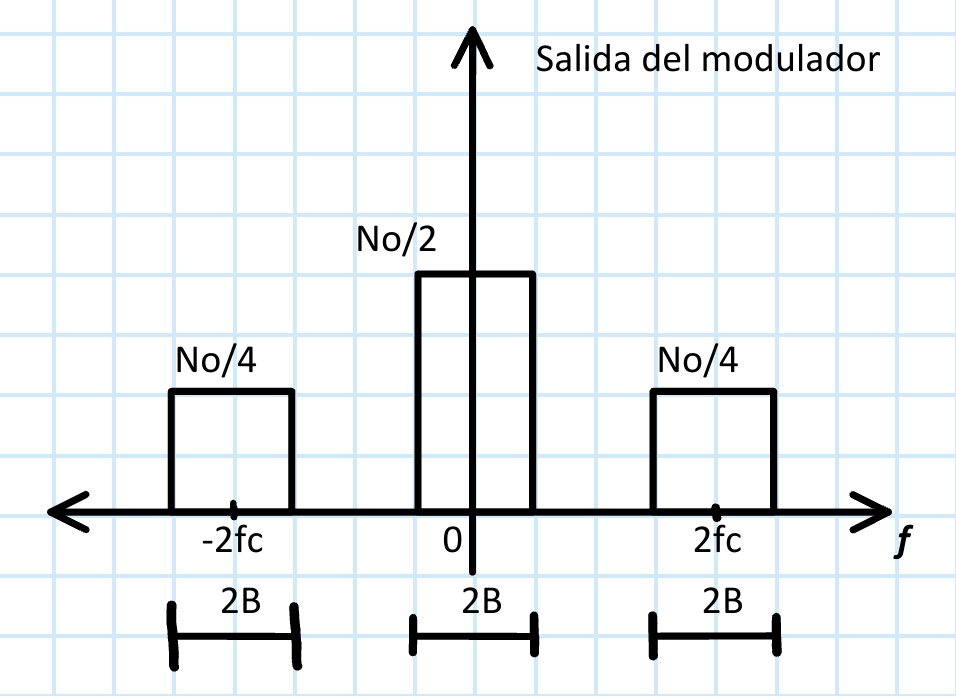
\includegraphics[width=7cm]{parte_teorica/actividad6_modulador.jpg}
			\caption{Densidad espectral salida modulador.}
			\label{fig:6modulador}
		\end{figure}



	\noindent Finalmente, la salida del modulador producto ingresa al filtro pasabajo, por lo que la densidad espectral de potencia en la salida del 
	filtro pasabajo es:
		\[
				S_{N_{PasaBajo}}(f) =
				\begin{cases}
				\dfrac{N_0}{2} & -B < f < B \\[6pt]
				0 & \text{o.c.}
				\end{cases}
		\]

	\noindent El gráfico de la densidad espectral de potencia a la salida del filtro pasabajo se observa en la Fig. \ref{fig:6pasabajo}.
    
		\begin{figure}[H]
			\centering
			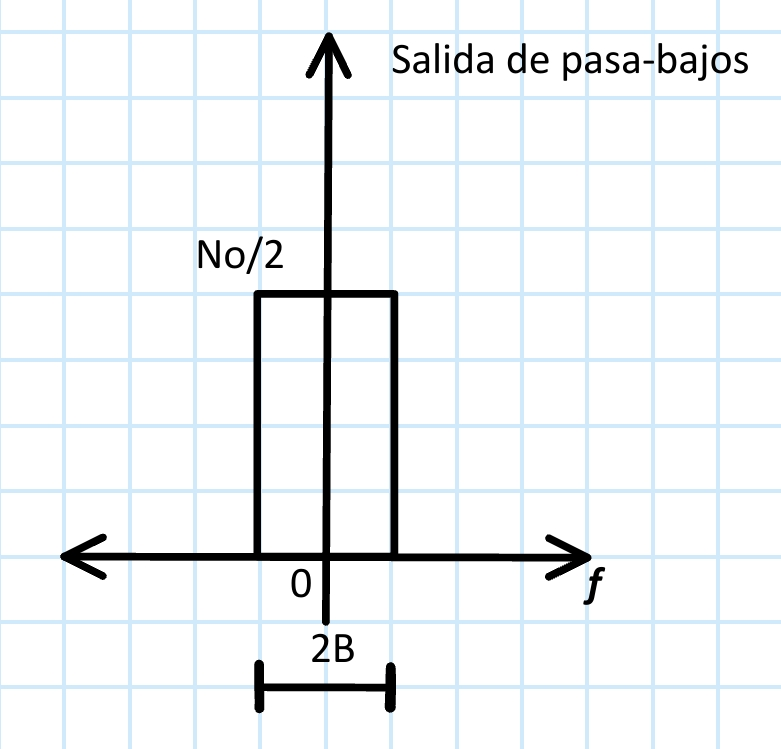
\includegraphics[width=7cm]{parte_teorica/actividad6_pasabajo.jpg}
			\caption{Densidad espectral salida filtro pasa bajo.}
			\label{fig:6pasabajo}
		\end{figure}

	\noindent La función de autocorrelación se obtiene a partir de la transformada inversa de la densidad espectral de potencia, es decir:
		\[
			R_{n(t)}(\tau) = \int_{-\infty}^{\infty} S_{N_{PasaBajo}}(f) e^{j 2 \pi f \tau} df
		\]
	\noindent Reemplazando la densidad espectral de potencia obtenida en la salida del filtro pasabajo, se tiene:
		\[
			R_{n(t)}(\tau) = \int_{-B}^{B} \dfrac{N_0}{2} e^{j 2 \pi f \tau} df
		\]
	\noindent Resolviendo la integral se obtiene:
		\[
			R_{n(t)}(\tau) = N_0 B \, \text{sinc}(2 B \tau)
		\]
	

\noindent b) Calcular la media y la varianza de n(t).\par
\bigskip

\noindent El ruido blanco gaussiano de entrada tiene media cero, y los filtros lineales e invariantes en el tiempo (filtro pasa banda y filtro
	pasa bajo) no alteran la media si la entrada tiene media cero. Esto se deduce de la siguiene ecuación:
	
		\[
			\mu_Y = \mu_X \int_{-\infty}^{\infty} h(\tau_1)\, d\tau_1 = \mu_X H(0)
		\]

	\noindent Por lo tanto, como la media $\mu_x$ dell ruido en la entrada es cero , entonces la media de $n(t)$ es:
		\[
			\mu_{n(t)} = \mu_x H(0) = 0 \cdot 1 = 0
		\]
	
	\noindent Para calcular la varianza se utiliza la siguiente ecuación:

		\[
		\sigma_x^2 = E[x^2] - \mu_x^2
		\]

	\noindent Por propiedad de autocorrelación se tiene que \(R_x(0) = E[x^2]\), reemplazando se obtiene lo siguiente:

		\[
		\sigma_x^2 = R_x(0) - 0 = N_0 B \, \text{sinc}(0)
		\]

		\[
		\sigma_x^2 = N_0 B
		\]


\noindent c) ¿Cuál es la tasa a la cual $n(t)$ puede ser muestreada, de manera tal de que las muestras resultantes sean no correlacionadas? \par
\bigskip

\noindent Se busca que la función de autocorrelación sea igual a 0. Entonces, teniendo en cuenta la Ecuación 8, 
esta función da 0 cuando el valor dentro del seno cardinal es un entero

	\[
		2B\tau = k, \quad k \in \mathbb{Z}
	\]

\noindent Entonces

	\[
		f_{\text{muestreo}} = \frac{k}{2B}
	\]

	\[
		T_{\text{muestreo}} = \frac{2B}{k}
	\]

\noindent Por lo tanto, la tasa de \(n(t)\) debe ser al menos \(2B\) muestras por segundo para que las muestras 
resultantes sean no correlacionadas.
